

\begin{figure}[h!]
	\centering
 	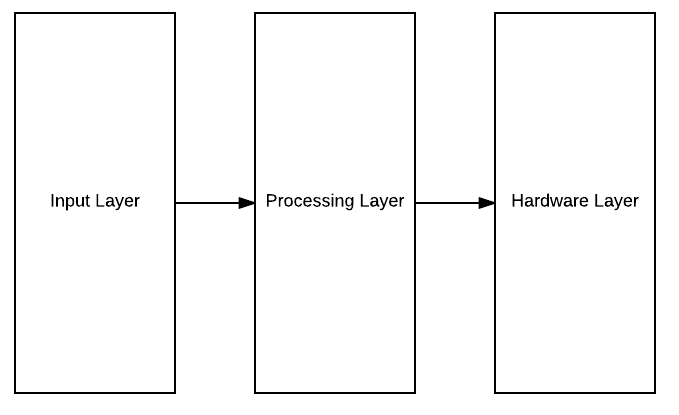
\includegraphics[width=0.60\textwidth]{images/layer_diagram}
 \caption{A simple architectural layer diagram}
\end{figure}

\subsection{Input Layer}


The input layer is the layer that receives information. It is comprised of the user interface and the camera input and is responsible for communicating commands to the Openrave simulation. From this layer, the user will be able to view the simulation running, the camera feed, motor positions and controls. This layer will be run on the minnow board on Ubuntu

\subsection{Processing Layer}

The processing layer is run on OpenRave and the C Code on the Teensy. This layer will be what moves the robot arm hardware as well as receive commands and provides simulation data and position data to the application layer. In OpenRave, the processing will calculate the kinematics and optimal movement for the robot arm, and the C Code on the Teensy board is what sends commands to the hardware layer

\subsection{Hardware Layer}

The hardware layer comprises of the skeletal arm, the motors, the encoders, the linear actuator, and the air pump. This layer will be carrying out the commands and operating the physical process or sorting objects and arm movement, and the pick and place operation. This layer receives the motor step commands as well as the commands for the end effector to pick up and place objects, and returns the encoder positions and linear actuator positions to the application layer.

